\documentclass[12pt,a4paper]{article}
\usepackage{lipsum}
\usepackage[T1]{fontenc}
\usepackage[utf8]{inputenc}
\usepackage[noadjust]{cite}
\usepackage{authblk}
\usepackage[top=1in, bottom=1in, left=1in, right=1in]{geometry}
\usepackage{fancyhdr}
\usepackage{listings}
\usepackage{csquotes}
\usepackage{color}
\usepackage{setspace}
\usepackage{url}
\usepackage{graphicx}
\usepackage{float}
\usepackage{tabularx}
\graphicspath{ {img/} }

\definecolor{gray}{rgb}{0.5,0.5,0.5}
\definecolor{lightgray}{rgb}{0.9,0.9,0.9}
\definecolor{editorGray}{rgb}{0.95, 0.95, 0.95}
\definecolor{editorMauve}{rgb}{0.58,0,0.82}
\definecolor{editorGreen}{rgb}{0, 0.5, 0} % #007C00 -> rgb(0, 124, 0)
\definecolor{editorBrown}{rgb}{.75, 0.375, 0} % #FF7F00 -> rgb(239, 169, 0)

\lstdefinelanguage{JavaScript}{
	morekeywords={typeof, new, true, false, catch, function, return, null, catch, switch, var, if, in, while, do, else, case, break},
	morecomment=[s]{/*}{*/},
	morecomment=[l]//,
	morestring=[b]",
	morestring=[b]'
}
\lstdefinelanguage{Bio}{
	morekeywords={A,C,G,T,a,c,g,t},
	alsoletter={<>\/()}
	morecomment=[s]{/*}{*/},
	morecomment=[l]//,
	morestring=[b]",
	morestring=[b]'
}
\lstdefinelanguage{HTML5}{
	language=html,
	sensitive=true, 
	alsoletter={<>=-},
	otherkeywords={
		% HTML tags
		<html>, <head>, <title>, </title>, <meta, />, </head>, <body>,
		<canvas, \/canvas>, <script>, </script>, </body>, </html>, <!, html>, <style>, </style>, ><
	},  
	ndkeywords={
		% General
		=,
		% HTML attributes
		charset=, id=, width=, height=,
		% CSS properties
		border:, transform:, -moz-transform:, transition-duration:, transition-property:, transition-timing-function:
	},  
	morecomment=[s]{<!--}{-->},
	tag=[s]
}

\lstset{%
	% Basic design
	backgroundcolor=\color{editorGray},
	basicstyle={\small\ttfamily},   
	frame=l,
	% Line numbers
	xleftmargin={0.75cm},
	numbers=left,
	stepnumber=1,
	firstnumber=1,
	numberfirstline=true,
	% Code design   
	keywordstyle=\color{blue}\bfseries,
	commentstyle=\color{editorGreen}\ttfamily,
	ndkeywordstyle=\color{editorBrown}\bfseries,
	stringstyle=\color{editorMauve},
	% Code
	language=HTML5,
	alsolanguage=JavaScript,
	alsodigit={.:;},
	tabsize=2,
	showtabs=false,
	showspaces=false,
	showstringspaces=false,
	extendedchars=true,
	breaklines=true,        
	% Support for German umlauts
	literate=%
	{Ö}{{\"O}}1
	{Ä}{{\"A}}1
	{Ü}{{\"U}}1
	{ß}{{\ss}}1
	{ü}{{\"u}}1
	{ä}{{\"a}}1
	{ö}{{\"o}}1
}

%
\pagestyle{fancy}
\fancyhf{}
\fancyhead[R]{\thepage}
%\lhead{APPLICATION OF COMPUTATIONAL METHODS TO STUDY THE SELECTION OF AUTHENTIC AND CRYPTIC SPLICE SITES}
%\fancyhead[L]{\fontsize{7}{12} \selectfont APPLICATION OF COMPUTATIONAL METHODS TO STUDY THE SELECTION OF AUTHENTIC AND CRYPTIC SPLICE SITES}
\setlength{\parindent}{0ex}
%
\begin{document}
	%
	%title and author details
	
	\title{
	    {APPLICATION OF COMPUTATIONAL METHODS TO STUDY THE SELECTION OF AUTHENTIC AND CRYPTIC SPLICE SITES}\\~\\~\\
	    {\large A Project Report}\\
	    {\large Presented to}\\
	    {\large Dr. Sami Khuri}\\
	    {\large Department of Computer Science}\\
	    {\large San Jose State University}\\~\\~\\
	    {\large In Partial Fulfillment}\\
	    {\large of the Requirements for the Class}\\
	    {\large CS 298}\\~\\~\\
    }
    
    \author{By\\Tapomay Dey}
    \date{April 2017}
	\maketitle
	
	\thispagestyle{empty}
	
	\newpage
	\doublespacing
	\noindent
	\large ABSTRACT\\
	This report explains the significance of the process of splice site selection during the translation of pre-mRNA into proteins. This sets the premise for a very interesting and highly valuable problem of putative splice site detection. Our eventual goal is to better understand the mechanism by which cryptic splice sites are activated in presence of mutations at authentic splice sites. We try to address the research question whether we can predict putative splice sites using probabilistic models. This report explains the following three important machine learning algorithms: Decision trees, Random Forests, and Hidden Markov Models. The report also touches very lightly on recent advances in application of evolutionary algorithms to the general problem of splice site detection. The last section presents a hypothetical and intuitive analogy of how one may model the same problem using Convolutional Neural Network, a variant of Artificial Neural Network that is highly accurate in image recognition.
    
    \thispagestyle{empty}
	\newpage
	
	\tableofcontents
	\thispagestyle{empty}
	\newpage
	
	\clearpage
    \pagenumbering{arabic}
    \doublespacing
	\section{\large MOTIVATION}
    The eukaryotic genome consists of many genes. Transcription and translation are some of the important processes in the gene expression pathways. Transcription involves generation of messenger RNA (mRNA) from pre-messenger RNA (pre-mRNA). Both mRNA and pre-mRNA are sequences of nucleotides. The pre-mRNA is divided into nucleotide regions called Introns and Exons. An Exon-Intron boundary is called a 5’ splice site and an Intron-Exon boundary is called a 3’ splice spite. As per recent knowledge, the Introns are discarded and the Exons are stitched together to form the mRNA. \par
    The mRNA is the exact coding sequence(CDS) that is translated into proteins. Proteins comprise of sequences made from various combinations of twenty possible amino acids. Each of the twenty amino acids can be mapped to multiple nucleotide triplets (codons) from the mRNA. One of the first publications of these mappings was by Crick in The Origin of the Genetic Code [298.crick1]. The exact sequence of amino acids dictates the structural properties of the protein molecule. The structure and composition of a protein molecule influence the physical and chemical properties exhibited by the protein. These properties have been documented in the Wikipedia page on Amino Acids [297.25]. \par
	\begin{figure}[h]
		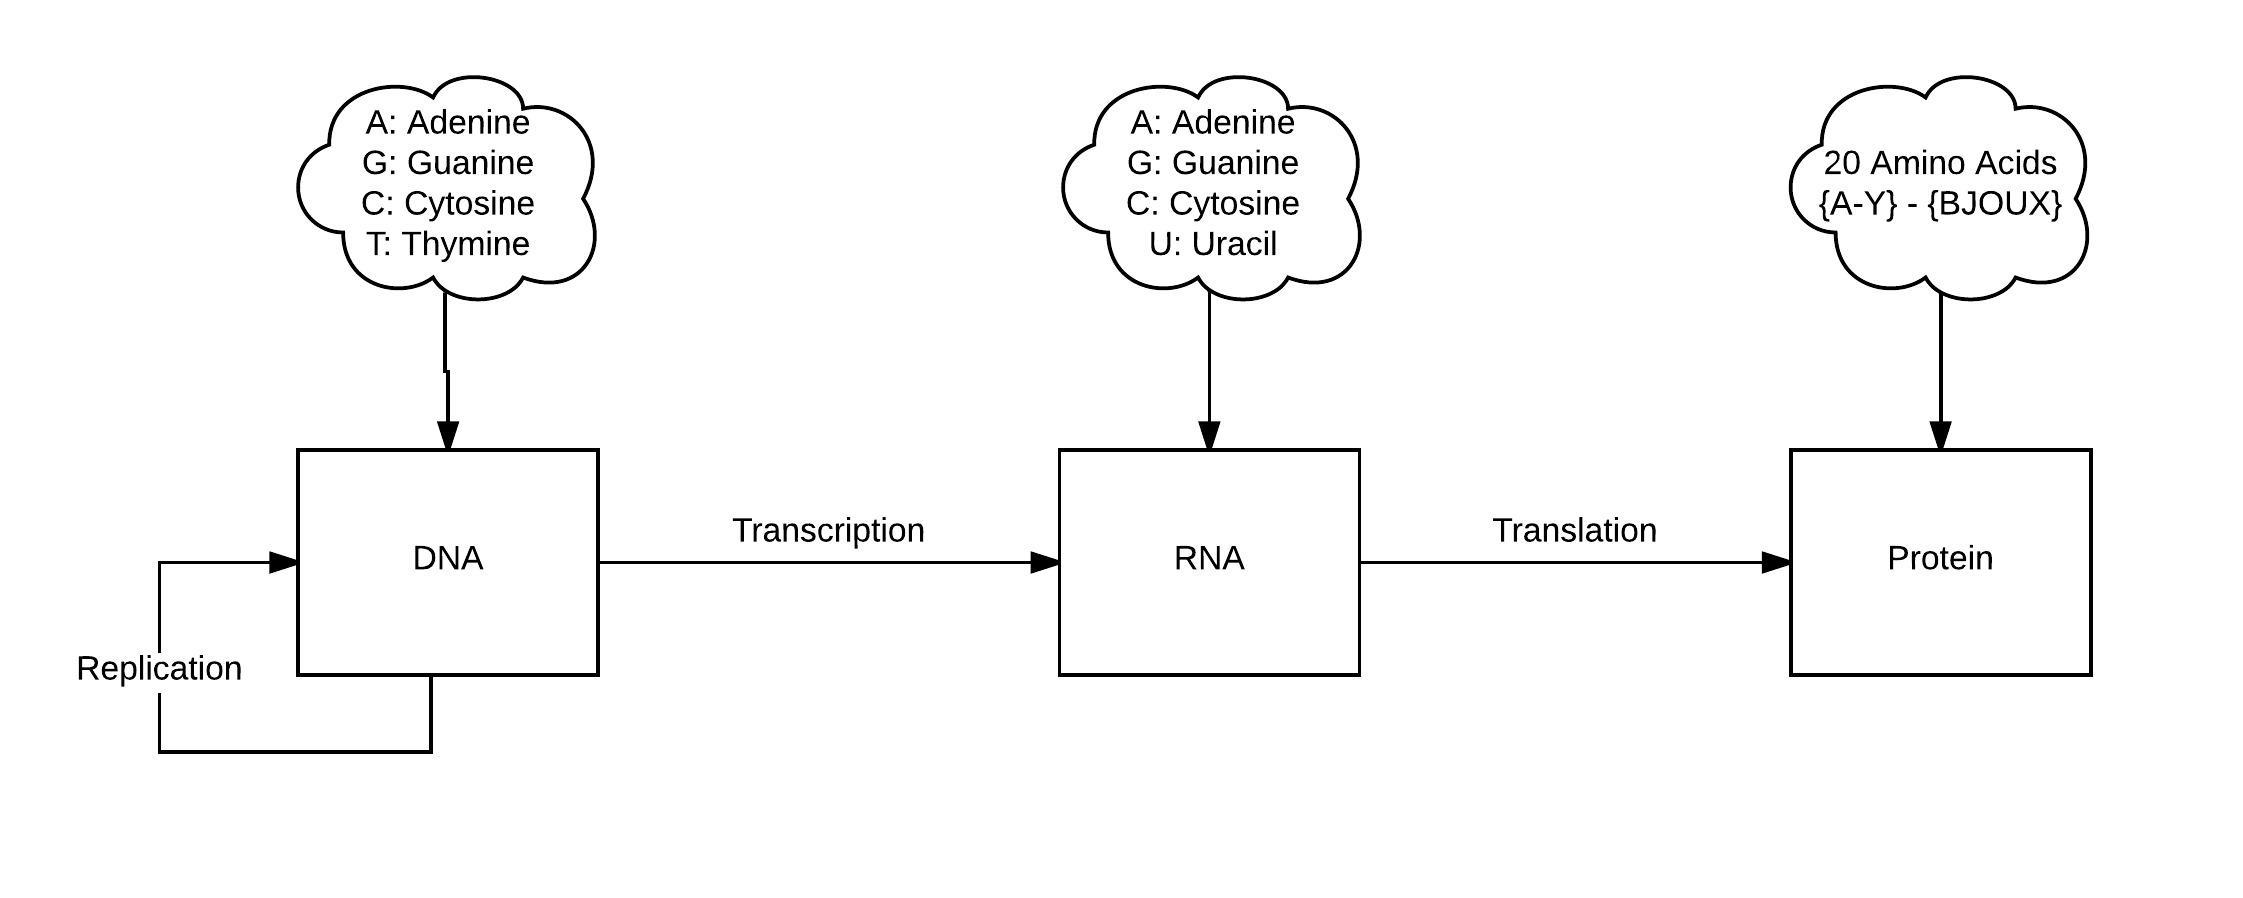
\includegraphics[width=\textwidth]{synthesis}
		\caption{Protein synthesis}
		\centering
	\end{figure}
	The proteins are responsible for various biological functions and traits of a eukaryotic organism. The splicing of pre-mRNA at 5’ and 3’ splice sites must be accurate in order to form the protein molecules that are required for satisfying the normally known functions of a healthy organism. \par
	Mutations in the DNA can lead to one of many possible disruptions in the selection of 5’ or 3’ splice sites. An obviously devastating disruption is a frame shift while extracting codons from the mRNA to form amino acid molecules. This may lead to a severely deficient expression of an important protein due to early detection of stop codons. In many cases, this leads to undesired consequences like fatal diseases. As per recent estimates, it is known that up to 50\% of disease-causing mutations disrupt splicing. \par
	The splice sites that are selected due to mis-splicing are called cryptic splice sites. However, there are multiple nucleotide subsequences in the pre-mRNA that contain candidate splice sites. Consequently, it is of crucial importance to understand the reasons behind the cryptic splice site selection by the spliceosome.
	

	\section{\large PROBLEM STATEMENT}
	To study the selection of splice sites by the spliceosome, three data sets were built, consisting of authentic, cryptic, and neighboring 5’ splice sites. The data sets comprise of thousands of 9-mers: sequences that are 9 bases long. Authentic and cryptic splice sites are extracted from public datasets. The neighboring splice site 9-mers are extracted from 100 base-pairs downstream and 100 base-pairs upstream of each cryptic splice site. \par
	The primary goal is to build probabilistic models for each data set and quantitatively compare their similarities. The primary hypothesis is that the authentic and cryptic splice sites are inherently different. The secondary hypothesis is that the neighboring splice sites are more dissimilar than both authentic and cryptic splice sites. This should help us understand the behavior of a spliceosome when it chooses cryptic splice sites and discards neighboring splice sites when the authentic splice site has been altered.
    
    \section{DATA SPECIFICATIONS}
    \subsection{5' SPLICE SITES}
    The 5’ splice sites are extracted based on the location of the invariant GT dinucleotide. The authentic splice sites are extracted from the Homo Sapiens Splice Sites database (HS3D) [298.ref: http://www.sci.unisannio.it/docenti/rampone/]. The cryptic splice sites and neighboring splice sites are extracted from the DBASS5 database[298.ref]
   	\begin{figure}[h]
   		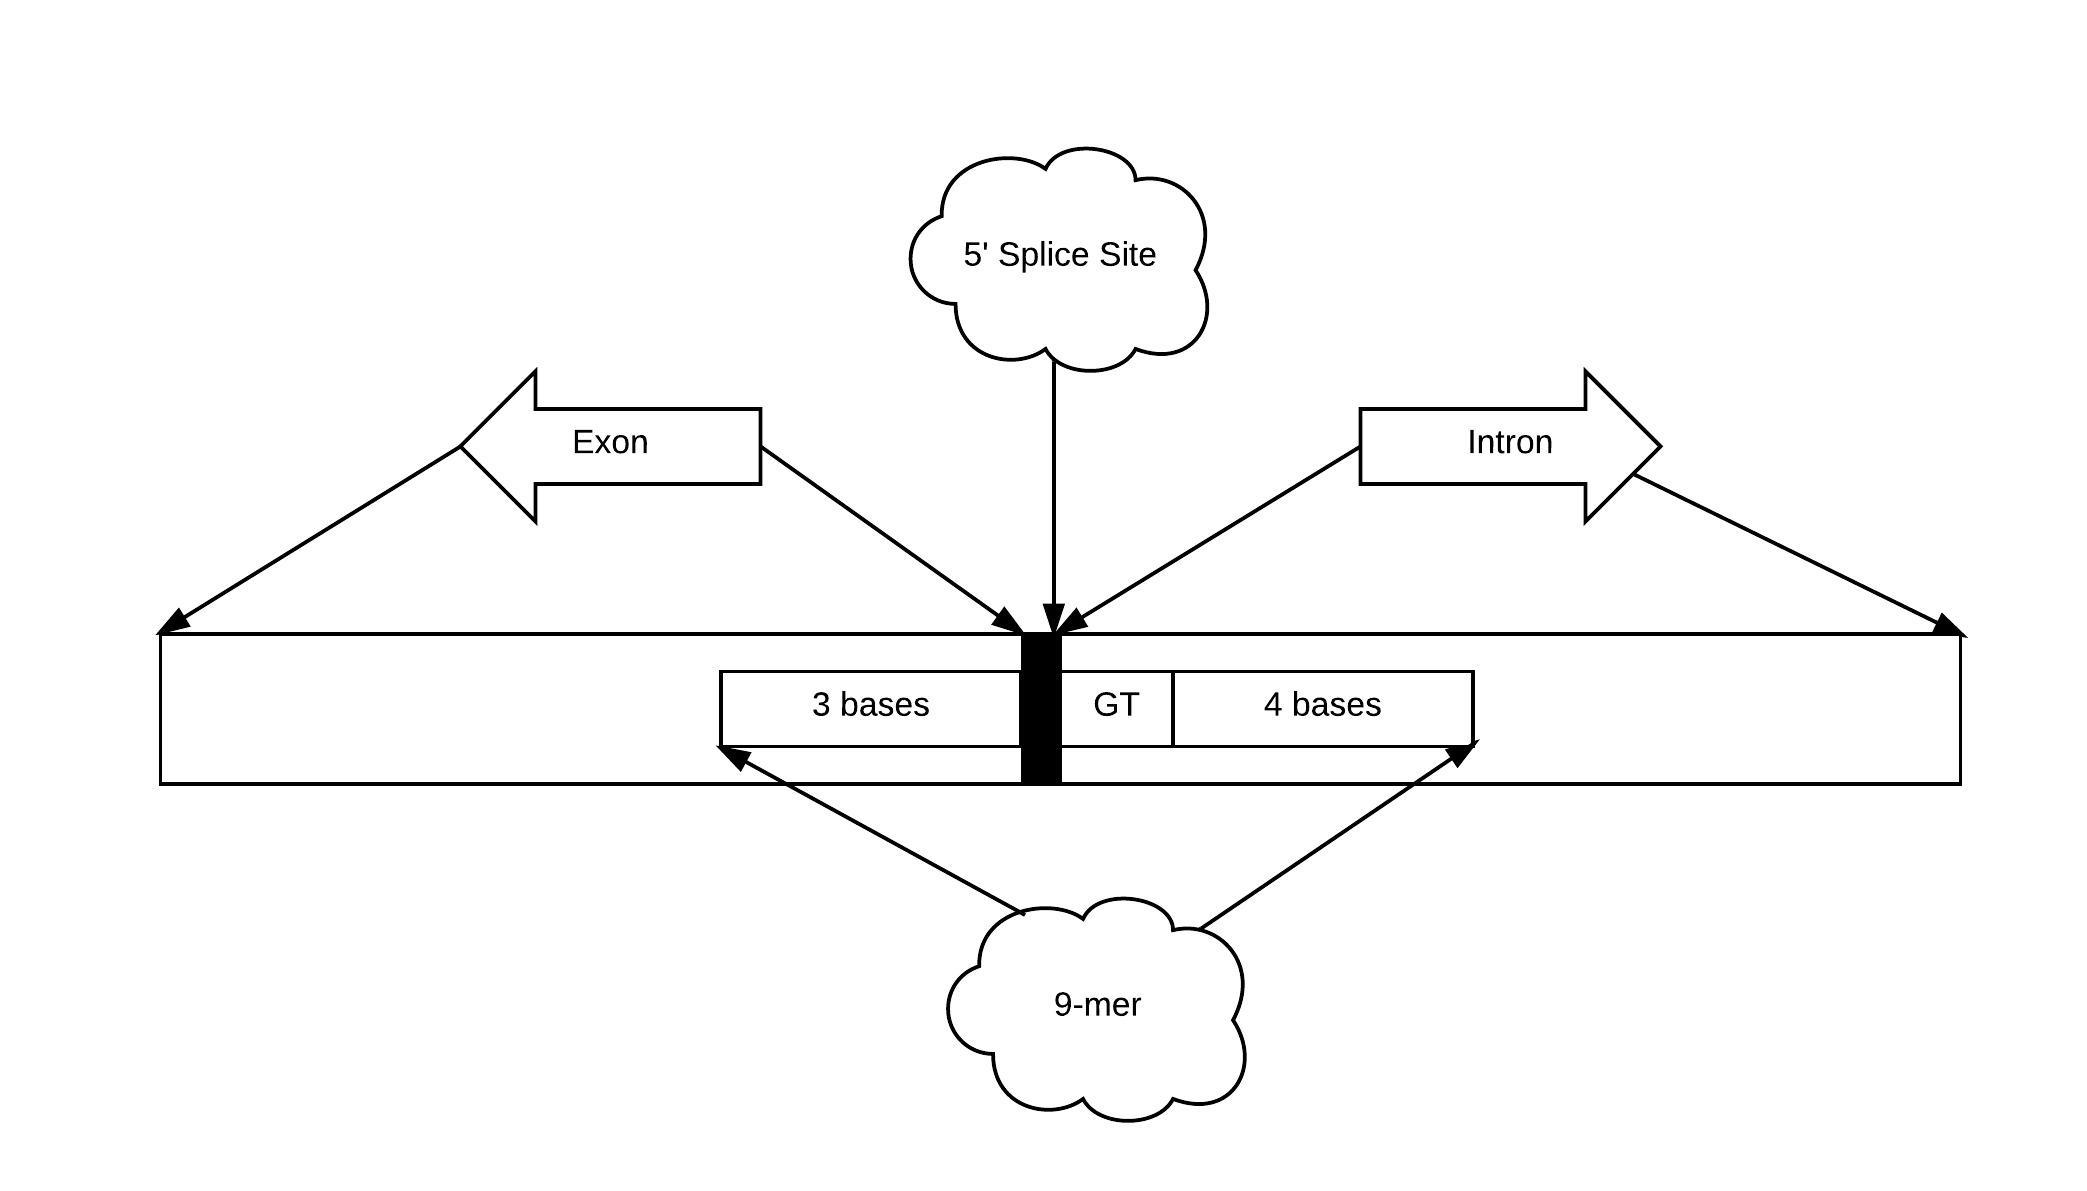
\includegraphics[width=\textwidth]{fiveprime}
   		\caption{5' Splice Site}
   		\centering
   	\end{figure}

	\subsection{AUTHENTIC 5' SPLICE SITE}
	HS3D offers the following files listed in [ref: Fig. hs3d\_download] for download:
   	\begin{figure}[H]
   		\includegraphics[width=\textwidth]{"hs3d_download"}
   		\caption{HS3D downloads page}
   		\centering
   	\end{figure}
	\par Since 5’ splice sites occur at the Exon-Intron boundary, the file EI\_true.zip is relevant for Authentic 5’ splice sites. The data is provided as an ‘seq’ file with 140 nucleotides in each line. Manually observing all the sequences reveals that the 5’ consensus GT dinucleotide that marks the start of the Intron is at position 71-72 in each sequence. The desired 5’ splice site 9-mer comprises of the last 3 nucleotides from the Exon, the GT dinucleotide from the start of Intron and the 4 nucleotides following it. \par
	Following is a sample of 9-mers extracted from the dataset:
	
	\begin{table}[H]
	\caption{Input sequence lines from file EI\_true.seq}
	\begin{tabular}{ | p{\linewidth} |}
		\hline
		AB000381  ( 1,2,2): CTCCTCTTTGCCTTACTCCTAGCCATGGAGCTC \newline
		CCATTGGTGGCAGCCAGTGCCACCATGCGCGCTC\textbf{AGTGTAAGT}\newline
		ATCATTCCCTCTCACTGTCCTGGAGAGGACGAGAATTCCACCT\newline
		GGGGTGCTGGGGGTCACTGGG \\
		\hline
		AB000381  ( 2,3,3): AATGACTTCAACTGTCCCAACATTAGAGTATGT \newline
		CCGTATCATATTAGGCGCTGTATGACAATCTCCA\textbf{TTCGTAAGT}\newline
		ACCTCTTGGTCATTTGGACACATTGTAGATTAGTCCCCTACCT\newline
		GGGTAGTTTCTGGGGCCAGGG \\
		\hline
        AB002059  ( 3,1,1): TGACCAGGAACTGGCGGGTGGGCGCCCTGCAGA \newline
		GGCTGCTGCAGTTTGGGATCGTGGTCTATGTGGT\textbf{AGGGTAAGA}\newline
		GAGAAGAGCTTTTGGCCAGGCTGGAGGGGCAAGGGAAGAGGTG\newline
		GGGGGTGGGGCTTGGTCCTGC \\
		\hline
		AB002059  ( 4,2,2): TTCCGTCACTCAGATCAAGGAGCTTGGAAACCG \newline
		GCTGTGGGATGTGGCCGACTTCGTGAAGCCACCT\textbf{CAGGTGGGG}\newline
		GCCCTGATGTTGCTGACGGGGGCGCAAGTCCTTTCCCCACTGA\newline
		CAGCCTGAACACCCGCCATGC \\
		\hline
	\end{tabular}
	\end{table}
	
	
	\begin{table}[H]		
		\caption{9-mers extracted from the sequences in Table 1}
		\begin{tabular}{ | c |}
			\hline
			AGT\textbf{GT}AAGT \\
			\hline
			TTC\textbf{GT}AAGT \\
			\hline
			AGG\textbf{GT}AAGA \\
			\hline
			CAG\textbf{GT}GGGG \\
			\hline
		\end{tabular}
		\centering		
	\end{table}
	
	Total authentic 5’ splice site 9-mers extracted : \textbf{2796}
	
	\subsection{CRYPTIC 5' SPLICE SITE}
	
	The cryptic 5’ splice sites are collected from the DBASS5 database portal [298.ref: http://www.dbass.org.uk/DBASS5] by crawling all available splice details page. The splice site details page contains the nucleotide sequence with the context of the mutation that alters the splicing location. The mutation is indicated in the sequence with a greater than symbol. \par
	For e.g: (G>A) means G is replaced by A \newline
	The cryptic splice sites are denoted by the slash symbol. \newline
	Consider the following nucleotide sequence extracted from the first record.\newline
	URL: http://www.dbass.org.uk/DBASS5/viewsplicesite.aspx?id=627 (last retrieved: 04/23/2017)

		
	\begin{tabular}{ | p{\linewidth} |}
		\hline
		CCAGCAACTT GGCTCTTTTT GGAGAGCGGC TGGGCCTGGT TGGCCACAGC CCCAGTTCTG CCAGCCTGAA CTTCCTCCAT GCCCTGGAGG TCATGTTCAA ATCCACCGTC CAGCTCATGT TCATGCCCAG GAGCCTGTCT CGCTGGACCA GCCCCAA\textbf{G/G} TGTGGAAGGA GCACTTTGAG GCCTGGGACT GCATCTTCCA GTAC\textbf{(G>A)}g tgaggccagg gacccgggca gtgctatggg gaagggacac catgggggcc caatttctcc ctctccacca cccagtgggg aatggaggcc acagggaggg gtcggggatt cctcaccttc ctgccaggga gattggtgcg aggctggggc tgggctgggc tgatccggag aatttgggat gagagcaggg agacttgggt gtcggggcag tctgggcagg aggaggacac tgaaggatgt ctcccagcac caaagtctga gggctgcctc ccgctccccg \\
		\hline
	\end{tabular}
	
	We can observe from other details on the page that:
	\begin{itemize}
		\item Capital nucleotide symbols indicate the trailing part of the Exon
		\item Small nucleotide symbols indicate the leading part of the Intron
		\item Mutation is marked as : (G>A)
		\item Cryptic splice site is marked as : “GCCCCAAG/G TGTGGAAGG”
	\end{itemize}
	The cryptic 5’ splice site 9-mer extracted from the above sequence is: AAGGTGTGG \par
	Total cryptic 5’ splice site 9-mers extracted : \textbf{539}

	\subsection{3' SPLICE SITE}
	The 3’ splice sites are extracted based on the location of the invariant AG dinucleotide and its preceeding Yn consensus were Y is a Pyridine. The authentic splice sites are extracted from the Homo Sapiens Splice Sites database (HS3D) [298.ref: http://www.sci.unisannio.it/docenti/rampone/]. The cryptic splice sites and neighboring splice sites are extracted from the DBASS3 database[298.ref]
   	\begin{figure}[H]
   		\includegraphics[width=\textwidth]{"threeprime"}
   		\caption{3' Splice Site}
   		\centering
   	\end{figure}

	\subsection{AUTHENTIC 3' SPLICE SITE}
	Since 3’ splice sites occur at the Intron-Exon boundary, the file IE\_true.zip is relevant for Authentic 3’ splice sites. This data is also provided as an ‘seq’ file with 140 nucleotides in each line. Manually observing all the sequences reveals that the 3’ consensus AG dinucleotide that marks the end of the Exon is at position 69-70 in each sequence. The desired 3’ splice site 13-mer comprises of the last 12 nucleotides from positions 59-70 at the end of the Exon, and one nucleotide from the start of the Intron. \par
	Following is a sample of 13-mers extracted from the dataset:

	\begin{table}[H]
		\caption{Input sequence lines from IE\_true.seq}
		\begin{tabular}{ | p{\linewidth} |}
			\hline
			AB000381(1,1,2): GGCCAGGGGCATAGAGCTGGCCAAGGAGCCATGGCTCAC\newline
			TAACGTGTTGTATGGGGCT\textbf{CCTTCCCTTCAGG}TCCAGGCTCCTGCGTGAAG\newline
			TGATGCTCCTCTTTGCCTTACTCCTAGCCATGGAGCTCCCATTGGTGGCA \\
			\hline
			AB000381(2,2,3): GAGTGAGCTGGTAATGGGTGGAAAAGGCGTAGTGGAGCA\newline
			GAAGCCTGAAGCCTGCTTT\textbf{CTCCCCTCTCAGG}GACTTACAGTTTGAGATGC\newline
			CATGACTGTGCGGTCATAAATGACTTCAACTGTCCCAACATTAGAGTATG \\
			\hline
			AB000381(3,3,4): TGTATGTGCCTCAATATTTACAAGCAGAAAATGTGAAAT\newline
			CAATTATTTTCATTGCTGC\textbf{TTCTTTTTTTAGG}CATAAATTCTCGTGAACTAC\newline
			TTGTTTATAAGAACTGTACAAACAACTGCACATTTGTATATGCAGCTGA \\
			\hline
			AB002059(4,1,2): GTAGGGCTCAGCTCCGCCCCTGTCACTACACGCTGGGGA\newline
			CACACCACACTGCCCGACT\textbf{TCTCCTCCCCAGG}TGGGCGCTCCTCGCCAAAAA\newline
			AGGCTACCAGGAGCGGGACCTGGAACCCCAGTTTTCCATCATCACCAAA \\
			\hline
			AB002059(5,2,3): AGGCTGCCGGCTTCCGGCCTTTCCAGTCAACACGAGCCC\newline
			AGCCAGGCCAACCTTGAGA\textbf{CTTGCCTCCTAGG}GAGAGAACGTGTTCTTCTTG\newline
			GTGACCAACTTCCTTGTGACGCCAGCCCAAGTTCAGGGCAGATGCCCAG \\
			\hline
		\end{tabular}
	\end{table}
	
	\begin{table}[H]	
		\caption{13-mers extracted from the sequences in Table 3}	
		\begin{tabular}{ | c |}
			\hline
			CCTTCCCTTC\textbf{AG}G \\
			\hline
			CTCCCCTCTC\textbf{AG}G \\
			\hline
			TTCTTTTTTT\textbf{AG}G \\
			\hline
			TCTCCTCCCC\textbf{AG}G \\
			\hline
			CTTGCCTCCT\textbf{AG}G \\
			\hline
		\end{tabular}
		\centering
	\end{table}

	Total authentic 3’ splice site 13-mers extracted : \textbf{2880}
	\subsection{CRYPTIC 3' SPLICE SITE}
	The cryptic 3’ splice sites are collected from the DBASS3 database portal [298.ref: http://www.dbass.org.uk/DBASS3] by crawling all available splice details page. The fields on the DBASS3 splice site details pages are similar to the ones on the DBASS5 pages. \par 
	The desired 13-mer comprises of : 
	\begin{itemize}
		\item 10 nucleotides before the ag dinucleotide from the Intron
		\item the ag dinucleotide at the splice site marker from the Intron
		\item one nucleotide after the splice site marker from the Exon
	\end{itemize}
	Consider the following nucleotide sequence extracted from a record at URL: http://www.dbass.org.uk/DBASS3/viewsplicesite.aspx?id=52 (last retrieved: 04/23/2017)\par
	\vspace{5mm}	
	\begin{tabular}{ | p{\linewidth} |}
		\hline
		gtaagggccg ggggcatttt ttctttctta aaaaaatttt tttttaagag atgggttctt gctatgctgc ccaggctggt cttaaattcc tagtctcaaa tgatcctccc acctcagcct caagtgtgag ccacctttgg ggcatcccca atccaggtcc ctggaagctc ttgggggggc atatctggtg gggagaaagc aggggttggg gaggccgaag aaggtcaggc cctcagctgc cttcatca\textbf{g/ t}tcccaccct cca\textbf{g/c}cccc \textbf{(a>g)}\textbf{(c>g)} ctcctcctgc agACAAGCTG GTGTCTAGGA ACTACCCGGA CCTGTCCTTG GGAGACTACT CCCTGCTCTG GAAAGCCCAC AAGAAGCTCA CCCGCTCAGC CCTGCTGCTG GGCATCCGTG ACTCCATGGA GCCAGTGGTG GAGCAGCTGA CCCAGGAGTT CTGTGAGgta \\
		\hline
	\end{tabular}
	\vspace{5mm} \break
	We can observe from other details on the page that:
	\begin{itemize}
	\item Capital nucleotide symbols indicate the leading part of the Exon
	\item Small nucleotide symbols indicate the trailing part of the Intron
	\item Mutations are marked as : (a>g) and (c>g)
	Cryptic splice sites are marked as : “cagctgc cttcatcag/ ttcccaccct ccag/cccc”
	\end{itemize}
	There are two cryptic 3’ splice site 9-mers extracted from the above sequence. They are: “tgccttcatcagt” and “cccaccctccagc” \par
	Total cryptic 3’ splice site 13-mers extracted : \textbf{306}

	\subsection{NEIGHBORING 5' SPLICE SITE}
	The putative splice sites around the known cryptic splice sites are called as neighboring splice sites. These are the putative splice sites that were not selected for splicing by the spliceosome in the event of a mutation. Using the nucleotide sequences extracted from the DBASS5 splice site details pages. The 100 base-pairs upstream and 100 base-pairs downstream of the splice site are parsed to look for the GT dinucleotide. All such occurrences are captured in the neighboring 5’ splice site dataset in the form of 9-mers with the GT dinucleotide as the 4th and 5th bases.\par
	
	Total neighboring 5’ splice site 9-mers extracted : \textbf{2213}
	
	\section{Algorithm selection}
	In case of 5’ splice sites, we can model the problem statement as a search problem. The spliceosome binds to a specific subset of the entire 9-mer search space. The cardinality of each position in the 9-mer is four (equivalent to A, C, G, and T), and the positions 4 and 5 are always occupied by the GT di-nucleotide. Hence, the size of the search space is $ 4^{7} = 16384 $. This search space comprises of the authentic, cryptic, and neighboring splice sites. An important goal is to study the statistical properties of the known samples from these three categories of splice sites and prove that they are inherently different. \par
	Evolutionary Algorithms(EAs) are applicable to problems that have no known classical optimization methods[handbook]. If a traditional method is applicable to solve a problem, then EA should not be used since traditional methods are more efficient in such a case. Since we do not understand the choices of a spliceosome completely, EAs are suitable for this problem. The section [Methods] describes a Genetic Algorithm based approach.\par
	Three primary forms of EA:
	\begin{itemize}
	\item Evolutionary Programming
	\item Genetic Algorithms
	\item Evolutionary Strategies
	\end{itemize}
	
	Some of the early significant contributors to EA:
	\begin{itemize}
	\item Friedberg(1958)
	\item Fraser(1957)
	\item Bremermann(1962)
	\item Box and Draper(1969): Evolutionary Operation
	\item Spendley(1962)
	\item Fogel(1966): Evolutionary Programming
	\item Holland(1967): Genetic Algorithms
	\item Rechenberg(1965): Evolutionary Strategies
	\end{itemize}
	
	Some of the initial conferences on EA:
	\begin{itemize}
	\item Schwefel and Manner(1991): Int'l workshop
	\item Belew and Booker(1991): ICGA'91
	\item Fogel and Atmar(1992): EP'92
	\item Manner and Manderick(1992): PPSN'92
	\end{itemize}
	
	\subsection{Background on Genetic Algorithms}
	Genetic Algorithms were first proposed and analyzed by John Holland(1975). Genetic Algorithms are a type of EA that deal with search and optimization based on a fitness function. It follows the philosophy of survival of the fittest. It uses the mechanisms of natural biological selection and genetics. \par
	Genetic algorithms follow a generic domain agnostic framework. Hence, it has the advantage of being applicable to many problems. Some of the features that initially separated GA from other evolutionary approaches are:
	\begin{itemize}	
	\item Bitstring representation
	\item Proportional selection
	\item Crossover
	\end{itemize}
	Although, the representation and selection methods have advanced significantly, there is still a large emphasis on the crossover operation. Crossover is known to give GAs a distinctive advantage over other methods[handbook]. \par
	
	%\renewcommand{\labelitemi}{$\textbullet$}
	General Terminology: \\
	- Population: A collection of individuals of size m \\
	- Individual: A single string of size m that is part of the population \par
   	\begin{figure}[H]
   		\includegraphics[width=\textwidth]{"population"}
   		\caption{Population and Individuals}
   		\centering
   	\end{figure}
	
	Biological terminology: \\
	- Generation: equivalent to a population \\
	- Chromosome: equivalent to an individual \\
	- Gene: Each of the n positions in a chromosome is called a gene. It can be treated as a variable and can take values from a fixed set of alleles \\
	- Allele: A fixed set of values that can be taken by a gene \par

   	\begin{figure}[H]
   		\includegraphics[width=\textwidth]{"generation"}
   		\caption{Chromosome, Gene, and Alleles}
   		\centering
   	\end{figure}

	Figure 7 shows a generic algorithmic framework for domain agnostic genetic algorithms. The selection strategy, fitness operator, crossover operator, and recombination strategy are customizable according to a need. The framework makes no assumptions about the initial population or the operators.
	
	\begin{figure}[H]
		\includegraphics[width=\textwidth,height=\textheight]{"GA-block1"}
		\caption{An algorithmic framework for genetic algorithms}
		\centering
	\end{figure}
	
	The two phases that can be used to introduce bias:
	\begin{itemize}
	\item Selection strategy
	\item Recombination / replacement strategy
	\end{itemize}
	
	\subsection{SELECTION STRATEGIES}
	Selection strategy is responsible for selecting individuals from a population for mating.
	\subsubsection{ROULETTE WHEEL}
	Total the fitness value of all individuals in the parent population; Calculate probability of each individual as the ratio of its fitness to total fitness. This strategy may lead to weak selection pressure. \par
	Selection pressure is governed by the differences in selection probabilities of individuals. If the differences are too small then the selection pressure is low.
	The workaround for low selection pressure is to scale the fitness probabilities with respect to the worst fitness. However, this leads to excessive selection pressure. The best individual may take over the entire population within a few iterations. \par
	
	\subsubsection{RANKED SELECTION}
	The workaround for excessive selection pressure is to use ranked selection. The parent population is sorted by fitness. Probability of selection is a linear function of the ranks sorted by fitness.
	
	\subsubsection{TOURNAMENT SELECTION}
	A small subset of the parent population is selected at random and the individual with best fitness is chosen for mating. This is repeated m times. The selection pressure can be controlled by adjusting the set size.
	
	\subsubsection{ELITIST STRATEGY}
	This is more of a strategy post selection. All but one of the child population after selection are chosen. The best individual from the parent population is added to the child population.
	
	\subsection{REPLACEMENT STRATEGIES}
	A child population is generated from the parent population P(t) using selection, crossover, and mutation operations. A suitable replacement strategy is required to form the population for the next generation P(t+1) using candidate individuals from both the parent and child populations.
	
	Some of the notable GA implementations that implement complex replacement strategies are:
	\begin{itemize}
	\item Whitleys GENITOR
	\item Syswerda’s steady-state GA
	\item Eshelman’s CHC
	\item Mühlenbein’s breeder GA
	\end{itemize}
	
	\subsubsection{REPLACEMENT STRATEGY ABSTRACTIONS}
	Let us assume:
	\begin{itemize}
	\item $\mu$: parent population
	\item $\lambda$: child population
	\end{itemize}
	
	\subsubsection{($\mu$ + $\lambda$) ES}
	The $\mu$ parents and $\lambda$ children are merged and the best $\mu$ individuals are chosen to form the new parent population.
	
	\subsubsection{($\mu$, $\lambda$) ES}
	The $\mu$ parents produce $\lambda$ offsprings such that $\lambda$ > $\mu$. The best $\mu$ offsprings out of the $\lambda$ offsprings are chosen to form the new parent population.
	
	\subsubsection{REPLACEMENT STRATEGY: OTHER VARIATIONS}
	Two other degrees of variation in a replacement strategy:
	\begin{itemize}
	\item Number of matings per iteration: \\
	Whether the GA produces one or two versus many ($\mu$) offsprings in each iteration; De Jong and Sarma (1993) claim that the main difference between variations in number of allowed matings is that a strategy with fewer matings leads to higher variance in performance.
	\item Whether the replacement strategy is biased or not: \\
	In case of an unbiased replacement strategy, if all the parents are replaced by the children, then we risk losing good individuals from the parent population for good. An advantage of this strategy is that the algorithm may wander out of a local minimum.
	\end{itemize}
	
	\subsubsection{MOST COMMON PRACTICAL REPLACEMENT STRATEGIES}[goldberg]
	\begin{itemize}
	\item Delete All: \\
	All the child population replaces the entire current population
	\item Steady-state: \\
	Only n members of the current population are replaced by members from the child population; The quantity n and the strategy for removal are parametrized
	\item Steady-state-no-duplicates: \\
	Same as the Steady-state strategy except that the algorithm checks for duplicates while introducing chromosomes from the child population into the current population
	\end{itemize}

	\subsection{MUTATION}
	Mutation is the mechanism for producing variations by randomly replacing one allele with another. A commonly used rate of mutation is one over length of the string.

	\subsection{CROSSOVER}
	Crossover combines features from two highly fit individuals. The individuals maybe highly fit due to different reasons. However, we do not know which features account for the high fitness. Hence, the features are combined at random. \par
	Types of crossover:
	\begin{itemize}
	\item One-point crossover
	\item Two-point crossover
	\item K-point crossover
	\item Uniform crossover
	\item Uniform order-based crossover
	\item Order-based crossover
	\item Partially matched crossover (PMX)
	\item Cycle crossover (CX)
	\end{itemize}

	For more details on each type of crossover, refer to how they are used with 9-mer data in section [modeling]

	\begin{figure}[H]
		\includegraphics[width=\textwidth,height=\textheight]{"GA-block2-algo"}
		\caption{Simple GA with one-point crossover, roulette wheel selection, and delete all strategy}
		\centering
	\end{figure}

For more details, refer how they are used with 9-mer data in section [modeling]

	\begin{table}[H]
		
		\begin{tabular}{ | c |}
			\hline
			AGT\textbf{GT}AAGT \\
			\hline
		\end{tabular}
		\centering
		\caption{Table template}
	\end{table}

	\begin{thebibliography}{9}
		
		\bibitem{arstechnica}
		Bright, P. (2016, Feb 10). 
		\textit{Moore’s law really is dead this time. Arstechnica. Retrieved from }	    			
		\url{http://arstechnica.com/information-technology/2016/02/moores-law-really-is-dead-this-time/}
		\bibitem{cormen}
		 Cormen, T. H. (2009). 
		 \textit{Introduction to algorithms. MIT press.}
		 
		\bibitem{hammond}
        Hammond, K., \& Michaelson, G. (Eds.). (2012).
		\textit{Research directions in parallel functional programming. Springer Science \& Business Media.}

		\bibitem{jones}
		Jones, M. P., \& Hudak, P. (1993). 
		\textit{Implicit and explicit parallel programming in Haskell. Disponível por FTP em nebula. systemsz. cs. yale. edu/pub/yale-fp/reports/RR-982. ps. Z (julho de 1999). [Online]. Available:}
		\url {http://cs-www.cs.yale.edu/publications/techreports/tr982.pdf}
		
		\bibitem{marlow}
		Marlow, S. (2012). 
		\textit{Parallel and concurrent programming in Haskell. In Central European Functional Programming School (pp. 339-401). Springer Berlin Heidelberg.
[Online]. Available: }			\url{http://community.haskell.org/~simonmar/par-tutorial-cadarache.pdf}
		
		\bibitem{marlow2011monad}
		Marlow, S., Newton, R., \& Peyton Jones, S. (2011, September). 
		\textit{A monad for deterministic parallelism. In ACM SIGPLAN Notices (Vol. 46, No. 12, pp. 71-82). ACM. [Online]. Available: }	\url{http://community.haskell.org/~simonmar/papers/monad-par.pdf}
		
		\bibitem{obradovic}
		Obradovic, D. (1998). 
		\textit{Structuring functional programs by using monads. [Online]. Available: }	\url{http://citeseerx.ist.psu.edu/viewdoc/download?doi=10.1.1.39.3974&rep=rep1&type=pdf}
		
		\bibitem{steele}
		Steele, G. (2009). 
		\textit{The Future is Parallel: What's a Programmer to do? Guy Steele's 2009 lecture on parallelism at M.I.T. [Online]. Available: }		\url{https://groups.csail.mit.edu/mac/users/gjs/6.945/readings/MITApril2009Steele.pdf}
		
		\end{thebibliography}
	
\end{document}
